\chapter{Wykład 4. Zarządzanie wiedzą w przedsiębiorstwie}

\section{Wiedza potrzebna w projekcie}
% strona 19

\subsection*{Wiedza deklaratywna:}
\begin{itemize}
\item Składniki metodyki PMBOK:
\begin{itemize}
\item pojęcia
\item role
\item procesy
\item dokumenty
\item obszary wiedzy
\end{itemize}
\item Istniejące rozwiązania problemu
\item Technologie, z których można skorzystać
\end{itemize}

\subsection*{Wiedza strukturalna:}
\begin{itemize}
\item struktura zależności pomiędzy elementami metodyki PMBOK
\item struktura bazy danych spełniającej wymagania
\item struktura oprogramowania, które chcemy wytworzyć
\end{itemize}

\subsection*{Wiedza proceduralna:}
\begin{itemize}
\item jak wygląda przepływ danych w projekcie
\item jakie są przypadki użycia
\item kiedy są tworzone poszczególne dokumenty
\item jak można wykorzystać dostępne technologie
\end{itemize}

% ===========================================================================

\section{Procesy wykorzystania produktu projektu}
% strona 34

\begin{figure}[!h]
\centering
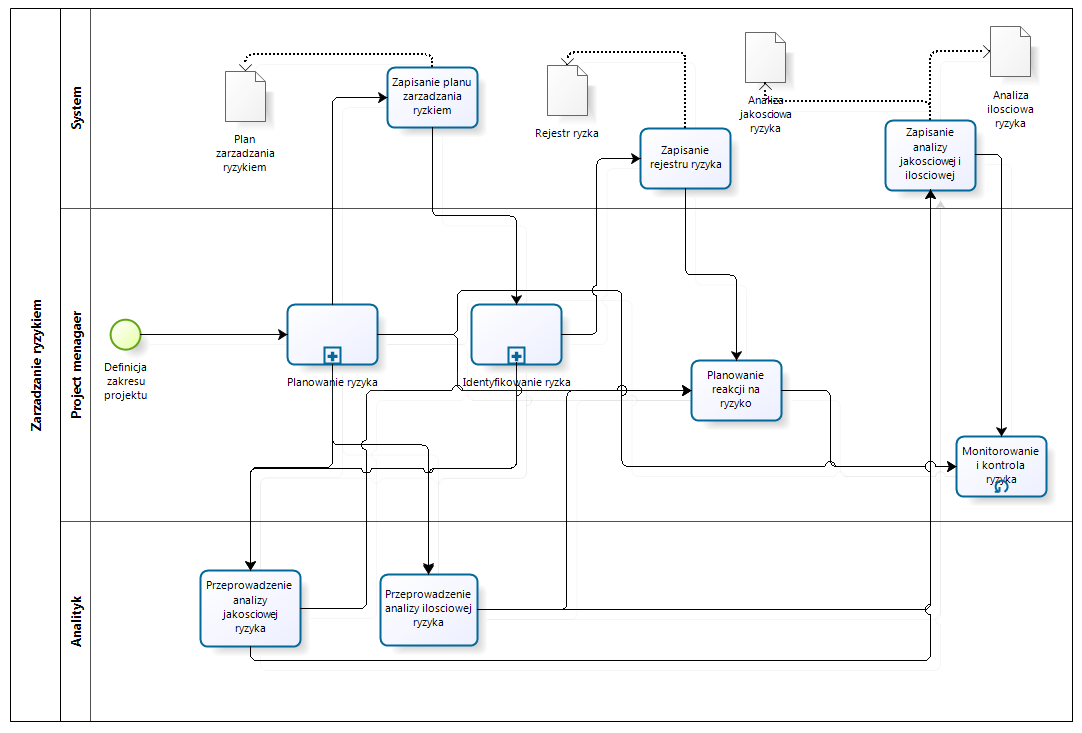
\includegraphics[width=1.1\textwidth]{zarzadzanieRyzykiem.png}
\caption{Zarządzanie ryzykiem}
\label{fig:zarzadzanieRyzykiem}
\end{figure}

\begin{figure}[!h]
\centering
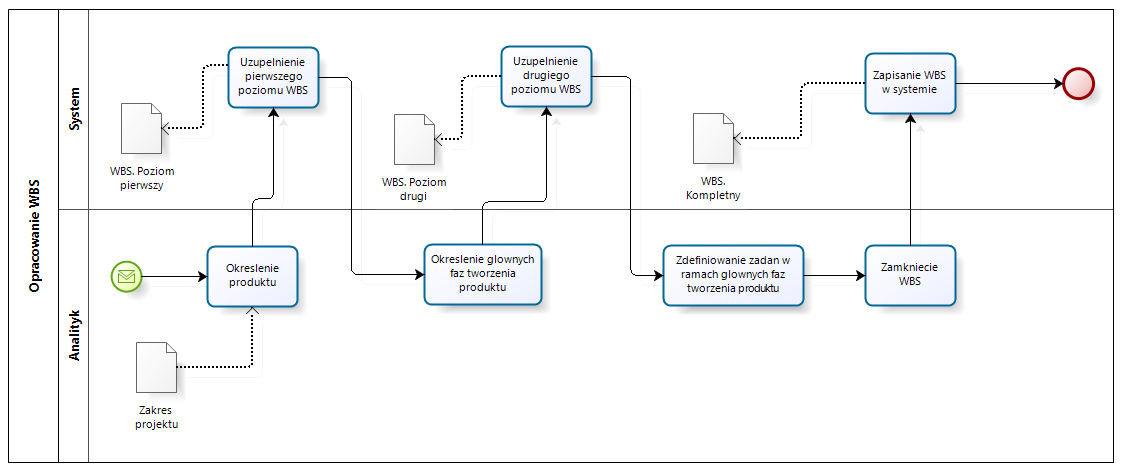
\includegraphics[width=1.1\textwidth]{opracowywanieWBS.png}
\caption{Tworzenie WBS}
\label{fig:opracowanieWBS}
\end{figure}

\clearpage

% ===========================================================================

\section{Systemy informatyczne do zarządzania wiedzą}
% strona 59

Do zarządzania wiedzą w przedsiębiorstwie można wykorzystywać różnorakie systemy. Ich najważniejszymi zadaniami są:
\begin{itemize}
\item Gromadzenie wiedzy
\item Systematyzacja wiedzy
\item Dystrybucja wiedzy
\end{itemize}

Przedstawione zostaną tutaj najważniejsze i najciekawsze z dostępnych programów.

\begin{itemize}
\item \textbf{Portale korporacyjne}. Najczęściej służą do jednokierunkowego przepływu informacji: od firmy do pracowników / klientów. Można rozszerzyć je o fora, albo dodać każdemu użytkownikowi możliwość dodawania informacji na portalu, jednak nie jest to skuteczny sposób na dwukierunkową komunikację.\\
\textbf{Przykładowe programy:} \textit{Drupal} (producent: Dries Buytaert), \textit{Joomla!} (producent: The OSM Development Team).

\item \textbf{Listy mailingowe}. Pozwalają na definiowanie grup, w ramach których wymieniane są informacje. Pozwala to na stworzenie prostego systemu przesyłania informacji w poszczególnych projektach (dla każdego projektu osobna lista). Można skorzystać z zewnętrznych serwerów, bądź zainstalować aplikację na firmowym sprzęcie. Są łatwo dostępne dla pracowników, dzięki możliwości obsługi przez przeglądarkę internetową. \\
\textbf{Przykładowe programy:} \textit{Google Groups} (zewnętrzny serwer), \textit{Majordomo} (producent: Great Circle Associates, do instalacji na własnym serwerze).

\item \textbf{Systemy zarządzania dokumentami (DMS)}. Umożliwiają gromadzenie i przeszukiwanie bazy dokumentów. Pozwalają na regulację dostępu poszczególnych osób do poszczególnych plików. Udostępniają również wersjonowanie wszystkich plików.\\
\textbf{Przykładowe programy:} \textit{Microsoft SharePoint}, \textit{OpenKM} (producent: GIT Consultors S.L.).

\item \textbf{Systemy automatyzacji pracy (workflow)}. Oprogramowanie takie pozwala na określenie ról poszczególnych osób w przetwarzaniu dokumentów oraz stanów pośrednich dokumentów. Procesy workflow przedstawia się zwykle w postaci grafu. \\
\textbf{Przykładowe programy:} \textit{Route} (OpenSource, tworzony przez Route Team), \textit{ONE Workflow} (producent: BeOne Sp. z o.o.).

\item \textbf{Bazy danych i hurtownie danych}. Pozwalają gromadzić bieżące dane, a także dane historyczne, na podstawie których przygotowywane są raporty i zestawienia.\\
\textbf{Przykładowe programy:} \textit{Microsoft Access}, \textit{LibreOffice Base} (producent: The Document Foundation).

\item \textbf{Systemy analizy danych (data mining)}. Pozwalają na odkrywanie powiązań pomiędzy danymi zapisanymi w bazach danych i hurtowniach danych.\\
\textbf{Przykładowe programy:} \textit{Oracle Data Mining}, \textit{Statistica: Data Miner} (producent: StatSoft).

\item \textbf{Wideokonferencje}.\\
\textbf{Przykładowe programy:} \textit{Skype} (producent: Microsoft), \textit{AQQ} (producent: CT Creative Team S.A.).

\item \textbf{Help-desk}. System umożliwiający zapisywanie i udostępnianie wiedzy zgromadzonej w procesie rozwiązywania problemów. W najprostszej wersji może to być podstrona portalu przedsiębiorstwa z listą najczęściej zadawanych pytań (FAQ).\\
\textbf{Przykładowe programy:} \textit{HelpTrac} (producent: Monarch Bay Software, Inc), \textit{Control-F1} (producent: CA Technologies).

\item \textbf{E-learning}. Nauka na odległość. Systemy pozwalające na przyswajanie wiedzy i kontakt z ekspertami poprzez internet.\\
\textbf{Przykładowe programy:} \textit{Moodle} (producent: Moodle Community), \textit{Chamilo} (producent: Chamilo Community).

\item \textbf{Systemy Wiki}. Typ witryn internetowych, w których treść można tworzyć i zmieniać w prosty i szybki sposób, z poziomu przeglądarki internetowej. Nie wymagana jest znajomość nawet HTMLa, ponieważ wykorzystywany jest specjalny język znaczników.\\
\textbf{Przykładowe programy:} \textit{MediaWiki} (producent: Wikimedia Foundation), \textit{DokuWiki} (producent: Andreas Gohr).

\item \textbf{Systemy ekspertowe}. Zawierają bazę wiedzy oraz reguły wnioskowania w celu rozwiązywania problemów.\\
\textbf{Przykładowe programy:} \textit{HeKaTe} (projekt rozwijany w Katedrze Automatyki), \textit{CLIPS} (stworzony przez NASA, aktualnie rozwijany przez CLIPS Expert System Group).

\end{itemize}

\clearpage

% ===========================================================================

\section{Mapa umysłu dla systemu zarządzania wiedzą}
% strona 70

\begin{figure}[!h]
\centering
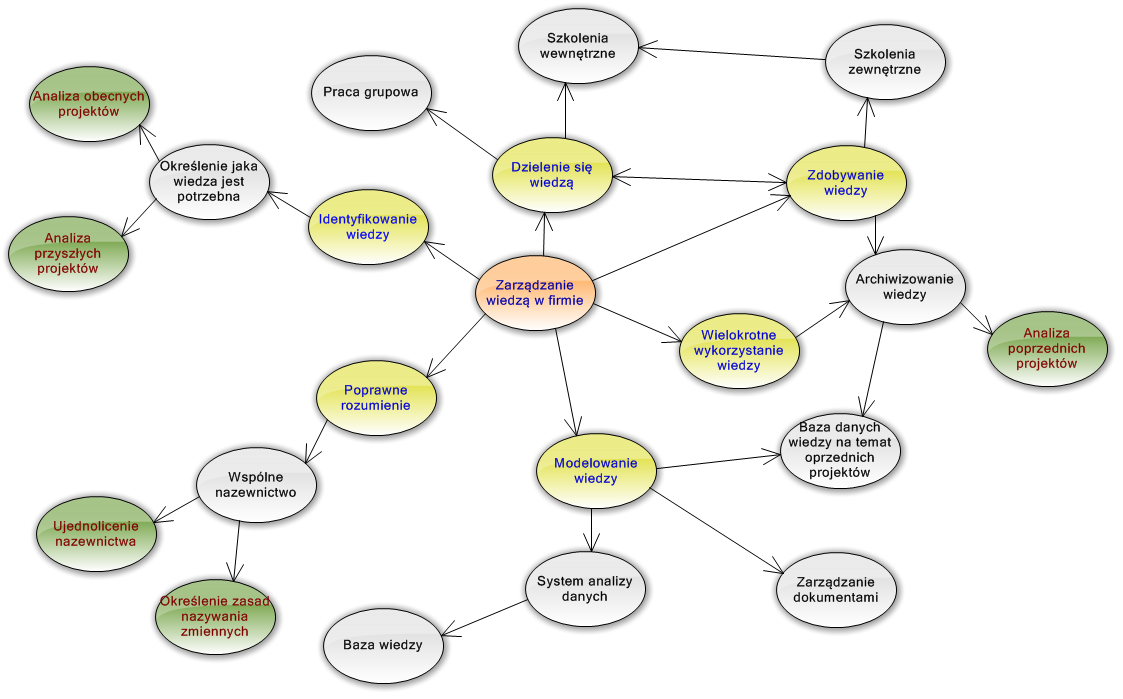
\includegraphics[width=\textwidth]{mapaMysli.png}
\caption{Mapa myśli}
\label{fig:mapaMysli}
\end{figure}

%\clearpage

% ===========================================================================

\section{Przegląd praktyk OPM3}
% strona 89

Praktyki OPM3, które powinny być w firmie:

\begin{enumerate}
\item Integrate PMBOK Guide Knowledge Areas; z racji związania projektu z metodyką PMBOK
\item Project Team Development Process Measurement; w związku z pracą zespołową nad projektem
\item Project Risk Response Planning Process Control; związane z występowaniem ryzyka
\end{enumerate}

Praktyki OPM3 zbędne w firmie:

\begin{enumerate}
\item Know Inter-Project Plan; w trakcie trwania projektu nie będą prowadzone równolegle inne projekty
\item Optimize Portfolio Management; brak portfolio
\item Track the Return of Investment; projekt nie jest inwestycją firmy
\end{enumerate}

